\documentclass[tikz,border=5mm]{standalone}
\usepackage{tikz}
\usetikzlibrary{arrows.meta, positioning, shapes.geometric, calc, backgrounds, fit, matrix, patterns, decorations.pathmorphing, shadows}

% --- COLOR DEFINITIONS ---
\definecolor{Garnet}{HTML}{73000A}
\definecolor{CSecondaryRed}{HTML}{CC2E40}
\definecolor{CBlue}{HTML}{466A9F}
\definecolor{CDark}{HTML}{1F414D}
\definecolor{COlive}{HTML}{65780B}
\definecolor{CLime}{HTML}{CED318}
\definecolor{CGold}{HTML}{A49137}
\definecolor{CGrayLight}{HTML}{E5E5E5}
\definecolor{CGrayDark}{HTML}{555555}
\definecolor{CWhite}{HTML}{FFFFFF}
\definecolor{CBlack}{HTML}{000000}

\begin{document}

\begin{tikzpicture}
    % Background glow
    \shade[inner color=CBlue!10, outer color=white] (-4,-2) rectangle (4,4);

    % Cam 1 (Static)
    \node[anchor=south] (C1) at (-2, 0) {
        \begin{tikzpicture}
            \fill[CWhite] (-0.5,0) rectangle (0.5, 1);
            \fill[CDark] (-0.5, 1) arc (180:0:0.5) -- cycle;
            \node at (0, -0.3) {Fixed};
        \end{tikzpicture}
    };
    
    % Cam 2 (Moving)
    \node[anchor=south] (C2) at (2, 0) {
        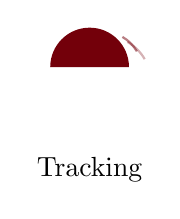
\begin{tikzpicture}
            \fill[CWhite] (-0.5,0) rectangle (0.5, 1);
            \fill[Garnet] (-0.5, 1) arc (180:0:0.5) -- cycle;
            % Motion blur lines
            \draw[Garnet, opacity=0.5, thick] (0.6, 1.2) arc (30:60:0.5);
            \draw[Garnet, opacity=0.3, thick] (0.7, 1.1) arc (30:60:0.6);
            \node at (0, -0.3) {Tracking};
        \end{tikzpicture}
    };
    
    \draw[ultra thick, gray] (-3, 0) -- (3, 0);
\end{tikzpicture}

\end{document}
